\section{CodeThorn Analysis Overview}

The analysis is performed in five phases

\begin{enumerate}
\item Syntactic and semantic analysis of the input program (ROSE). The program is analyzed and represented in memory as annotated abstract syntax tree (AST).
\item Control flow analysis. We compute a control flow graph (CFG) for the AST. Transitions, as computed for the state transition graph in the next phase, correspond to edges in the CFG.
\item General Data Flow analysis. We perform a data flow analysis with the general framework as described in \ref{section-algorithm}. During this analysis the state transition graph is computed.
\item LTL-Checking. Input to the LTL-Checking phase is the state transition graph and the LTL-formulae.
\item Reporting of analysis results. Assert reachability is computed based on the transition graph. Results for LTL-formulae are computed solely by the LTL-checker.
\end{enumerate}

Important properties of the perfomed analysis are

\begin{itemize}
\item The C files can be used unmofided (header files are analyzed as well).
\item The data-flow analysis does not require information about possible input values of a
  given program. All information, which is then represented in the
  transition graph, is extraced from the program code. The set of all
  possible input values is represented by the extracted constraint
  sets (as they are backpropagated from called functions to the
  main-function). The possible output values are represented in the
  property state as computed for the output operation (printf).
\item The LTL-Checker only depends on the extracted state transition graph.
\item We do not provide manually any information to the analyzer.
\end{itemize}

\subsection{System State}

A system state consists of a label (lab), a property state (pstate), a constraint set (cset), an IO property (io).

PState = Var $\rightarrow$ Val where Val is either a constant or top. Val is a lifted integer set.
SState = Lab x PState x Constraints x IO

Constraints is a set of constraints (see above).

IO determines whether one of the variables in PState is an input or output variable. More specifically, whether a variable is read from stdin, or printed to stdout or stderr. Furthermore it determines whether the state produces an output which is caused by a failed assert.

Labels are unique and represented as numbers. Ordering is therefore the same as for numbers.

Each constraints set is associated with an id. The id is used in PState.

Hence, the analysis information is represented as:

\begin{itemize}
\item Label: num
\item PState: VarId $\rightarrow$ Val
\item SState: Label $\times$ PStateId $\times$ ConstraintId $\times$ IOId
\end{itemize}

\subsection{Property States}

\fixme{describe property states, const-int-lattice}

\subsection{Minimal Constraint Sets}
A minimal constraint set (MCS) is a representation of
information about the variables and values with a minimal number of operators.

 The minimal number is
important for using a minimal amount of memory and for a proper
sorting criteria to be used in a sorted data structure (see section Implementation \ref{section-implementation})

The operators can range on variables and constants. Let x,y,z denote variables, and c, d constants with c!=d.
The constraints of interest are : 
\begin{itemize}
\item $x=c$: const-equality constraint
\item $x\neq c$, const-inequality constraint
\item $x=y$, var-equality constraint
\item $x\neq y$, var-inequality constraint (not used in RERS-problem analysis)
\end{itemize}

Additionally a set can be marked to represent a disequality, meaning that an equality and an inquality on the same variable have been added to the set. This is represented as \{\#\#\}.

Set union of $MCS_1$ and $MCS_2$ means inserting one constraint after another of $MCS_2$ into $MCS_1$.

Operators on constraints sets ensure the following properties of
constraint sets. Let a variable be denoted as x,y,z and constants be denoted as c, d.

\begin{itemize}
\item If an equality $x=c$ exists, then no inequality $x\neq c$ on x can exist.
\item There can exist at most on equality $x=c$ on the same variable.
\item Multiple inequalities $x \neq c_i$ can exist for a given variable. The number of inequalities is bound by constants extracted from conditions in the program.
\item If there exists at least one inequality $x\neq c_i$ then no equality $x=c_j$ can exist.
\item If there exists on variable-variable equality $x=y$ then constraints on x and y are not in conflict to above rules, as if x and y would be the same variable (otherwise the constraint set would be inconsistent).
\item Equalities and inequalities for different variables x and y, for which an euqality x=y exists, are never duplicated (i.e. renaming of variable y to x would not change the number of constraints in the constraint set)
\item If a variable-variable equality x=y is removed from the
  constraint set all constraints of those two variables x and y are
  duplicated to the other variable (.e.g. let the constraint set be
  ${x\neq 1, x=y, y\neq 2}$. If we remove the x=y constraint, then the
  set ${x\neq 1, x\neq 2, y\neq 1, y \neq 2}$ is obtained. In a
  subequent operation we may then remove all constraints of y. Such
  operations are performed on constraint sets when exiting the scope
  of local variables: in this case we remove the variable from the
  constraint set but do perform the information as above. This allows
  to propagate information about variables from a callee back to the
  caller in inter-procedural analysis. As a consequence, all
  constraints ``collected'' on the input variable as it is passed as
  argument in function calls are propagated from the entire program
  back to the main function. This information we use then in LTL
  checking, by using the value of the computed output variable and the
  constraints on the input variable.
\end{itemize}

Variable-Const equalities, $x=c$, and inequalites $x\neq c$, are
extracted from conditions. Variable-variable constraints are
introduced only by argument passing in functions calls (assignments do
not create $x=y$ constraints).

The extraction of constraints from conditions is crucial to our
Const-Int analysis. We therefore describe it in more detail in the
next section.

\subsection{Exact Constraint Extraction}

For the language subset as used in RERS-Problems 1-9 we denote this
language subset only consisting of assignments, equality and
inequality comparisons, function calls, and parameter passing, single
variable input and output, as RERS-ConstInt language subset.

With the following method we are able to extract exact const-int
equality and inequality constraints from a given RERS-ConstInt
program. We shall denote these constraints EQIQ-constraints. With
``exact'' we mean, that no more EQIQ constraints can be extracted from
the given program which would allow to represent more information
about the values in a variable for which no concrete value is know,
i.e. we use this information for reasoning on the input variable.

\fixme {more to come}

\subsection{IO Property - Input/Output and Exit Information}

This property represents the information that the operation is either
an input, an output, or a failed-assert operation. From the label and
the associated statement, details as relevant to reporting the
analysis results can be extracted. For example, in the RERS-problems
we find the information for a failed-assert by a) using the label to
find the corresponding statement and b) the associated C error label
is then found in a look-up operation on the ROSE AST.

\section{The State Transition Graph}

\newcommand{\deqop}[0]{\#\#}
\newcommand{\eq}[0]{=}

The State Transition Graph is a graph where nodes represent system states
and edges represent the transition between two states as computed by
the evaluations of the respective transfer function. They are
therefore annotated with the respective statement which has been
analyzed by the transfer function.

In the RERS challenge we use our ConstInt Analysis. This analysis is a
variation of constant propagation. The algorithm, as described in
\ref{section-algorithm} for computing system states uses the
following system state representation

\begin{itemize}
  \item a label: the respective label from the control flow graph
  \item a variable-property State: a mapping from variables to a
    lifted lattice of integers.
  \item a constraint set: a set of equality and inequality
    constraints. Additionally a constraint set can also represent a
    disequality (.i.e. the top element of the constraint lattice).
  \item an IO property: Input, Output and Exit information of the
    program. 
 \end{itemize}

\subsection{Folded System State Transition Graph}

The folded transition graph represents the same information as the state transition graph but is folded with respect to the label of each transition. The main purpose is visualization and presentation to the user.

\begin{figure*}[t]
\centering
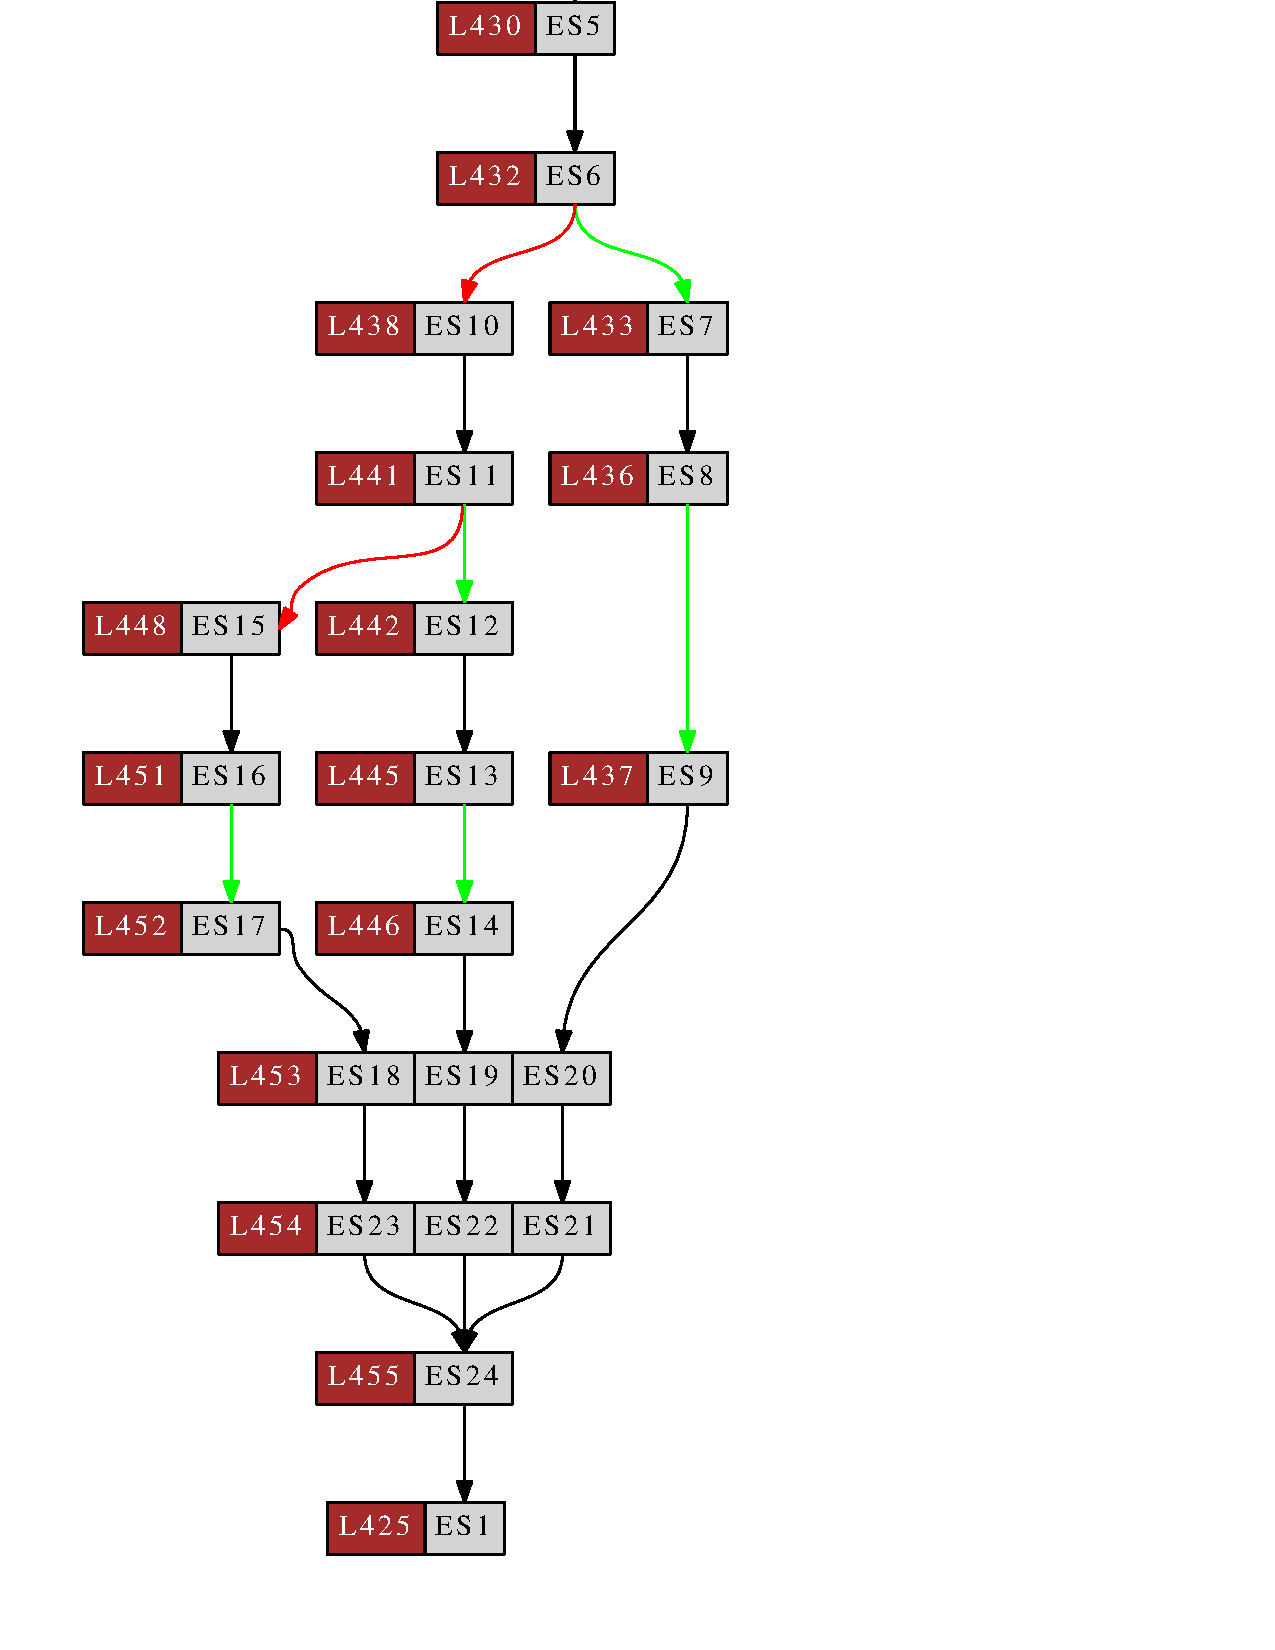
\includegraphics[width=0.7\textwidth]{gfx/basictest15_transitiongraph2.pdf}
\caption{Folded System State Transition Graph}
\end{figure*}

\begin{figure*}[t]
\centering
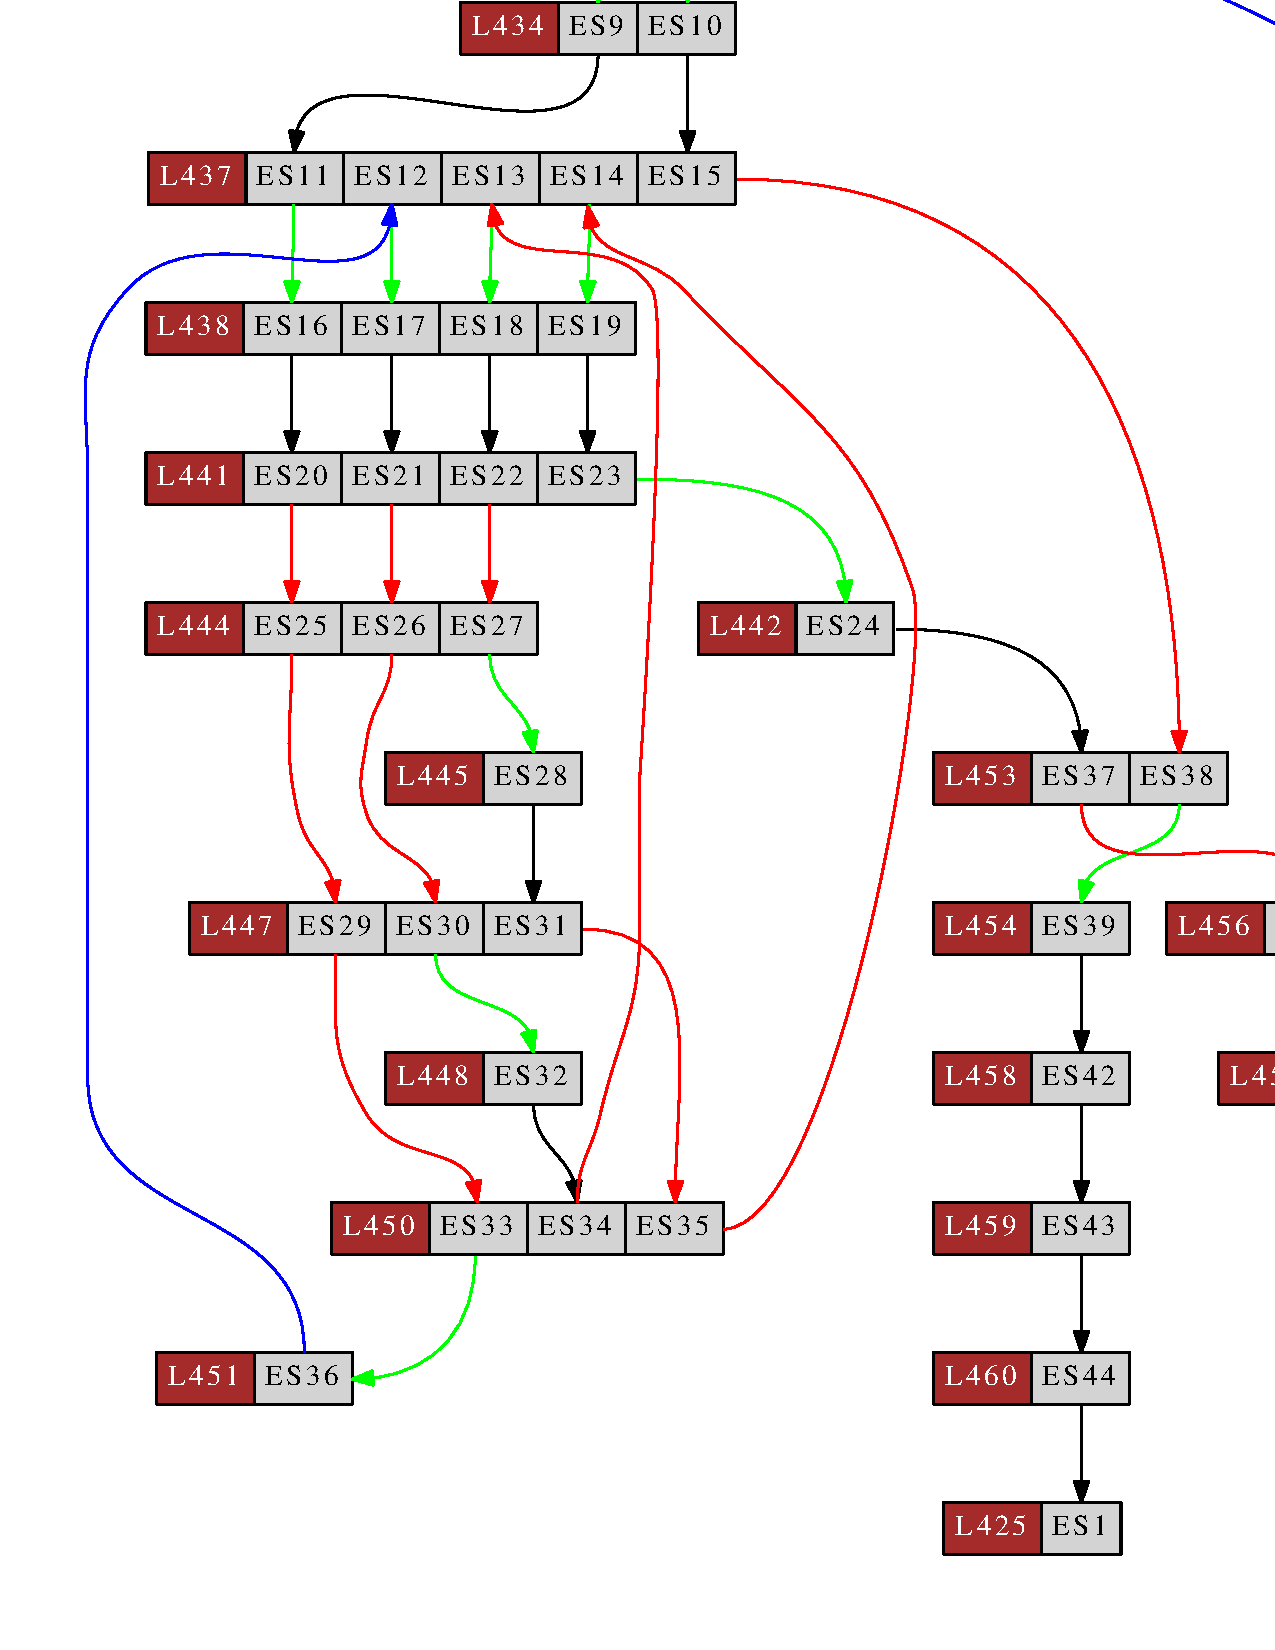
\includegraphics[width=0.7\textwidth]{gfx/basictest10f_transitiongraph2.pdf}
\caption{Folded System State Transition Graph (needs to reduced in size)}
\end{figure*}

\clearpage

\section{Solver and Algorithm}
\label{section-algorithm}

\fixme{describe algorithm}

\section{Implementation}
\label{section-implementation}

\fixme{describe data organization, approach for reducing redundancy, etc.}

A PState is sorted by the order of the variables ids.
PState$\eq$ PState: two PStates are equal if all variable bindings are equal.
PState$<$ one PState is smaller than another if, considering the sequence of variables as a string, the string is smaller than the other according to lexical order.

\section{Measurments}

\fixme{provide csv-timing output here}

\section{Conclusion}

\fixme{first you have to finish to finish first}
